%-----------------------circuit 2--------------------------
\section{Single Phase Half Wave Uncontrolled Rectifier with RL load}

\subsection{Circuit used for simulation}

% figure that is centered on the page
\begin{figure}[h]
    \centering
    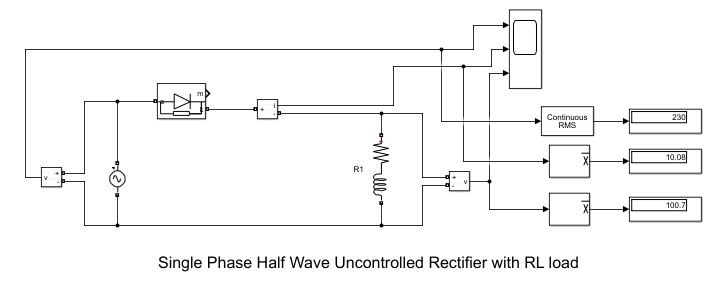
\includegraphics[width=0.7\textwidth]{images/experiment-1/circuit-diagram-simulation-02.png}
    \caption{Circuit used for simulation}
    \label{Fig_simulation_circuit_single-phase-half-wave-uncontrolled-rectifier-with-RL-load}
\end{figure}

\subsection{Components Required}

\begin{table}[h]
    \renewcommand{\arraystretch}{1.3}
    \label{table_components_required_circuit_2}
    \centering
    \begin{tabular}{|c|c|c|c|}
        \hline
        Sr. No & Parameters                     & Ratings            & Quantity \\
        \hline
        \hline
        1      & AC Single Phase Voltage Source & 230V ($ V_{rms} $) & 1        \\
        \hline
        2      & Resistor                       & 10$ \Omega $       & 1        \\
        \hline
        3      & Inductor                       & 10mH               & 1        \\
        \hline
        4      & Diode                          & -                  & 1        \\
        \hline
        5      & Voltmeter                      & -                  & 2        \\
        \hline
        6      & Ammeter                        & -                  & 1        \\
        \hline
    \end{tabular}
    \caption{Components for Single Phase Half Wave Uncontrolled Rectifier with RL load}
\end{table}


\subsection{Observations}

\begin{table}[h]
    \renewcommand{\arraystretch}{1.3}
    \label{table_observation_2}
    \centering
    \begin{tabular}{|c|c|c|}
        \hline
        Parameters                              & Theoretical Values & Simulation Values \\
        \hline
        \hline
        AC Input Voltage ($ V_{in,rms} $)       & 230V               & 230V              \\
        \hline
        Output Average Voltage ($ V_{o,avg} $)  & 103.53V            & 100.7V            \\
        \hline
        Output Average Current ($ I_{o,avg}  $) & 10.35A             & 10.08A            \\
        \hline
        AC Input Power ($ P_{AC} $)             & 2389.5 (W)         & 2435 (W)          \\
        \hline
        DC Input Power ($ P_{DC} $)             & 1071.53 (W)        & 1015 (W)          \\
        \hline
        Efficiency (\%)                         & 44.84              & 41.66             \\
        \hline
    \end{tabular}
    \caption{Observations for Single Phase Half Wave Uncontrolled Rectifier with RL load}

\end{table}


Upon observation, it is noted that the simulated values exhibit a level of conformity with the theoretical values. Due to the presence of an inductive component in the load, the output current lags behind the output voltage, resulting in a period during which the output voltage becomes negative while the diode conducts until the output current attains a value of zero. The diode then ceases to conduct, and both the output voltage and current return to zero.
The efficiency of uncontrolled rectifier with RL load is 41.66\%.
\pagebreak


\subsection{Resultant Waveforms}

% figure that is centered on the page
\begin{figure}[h]
    \centering
    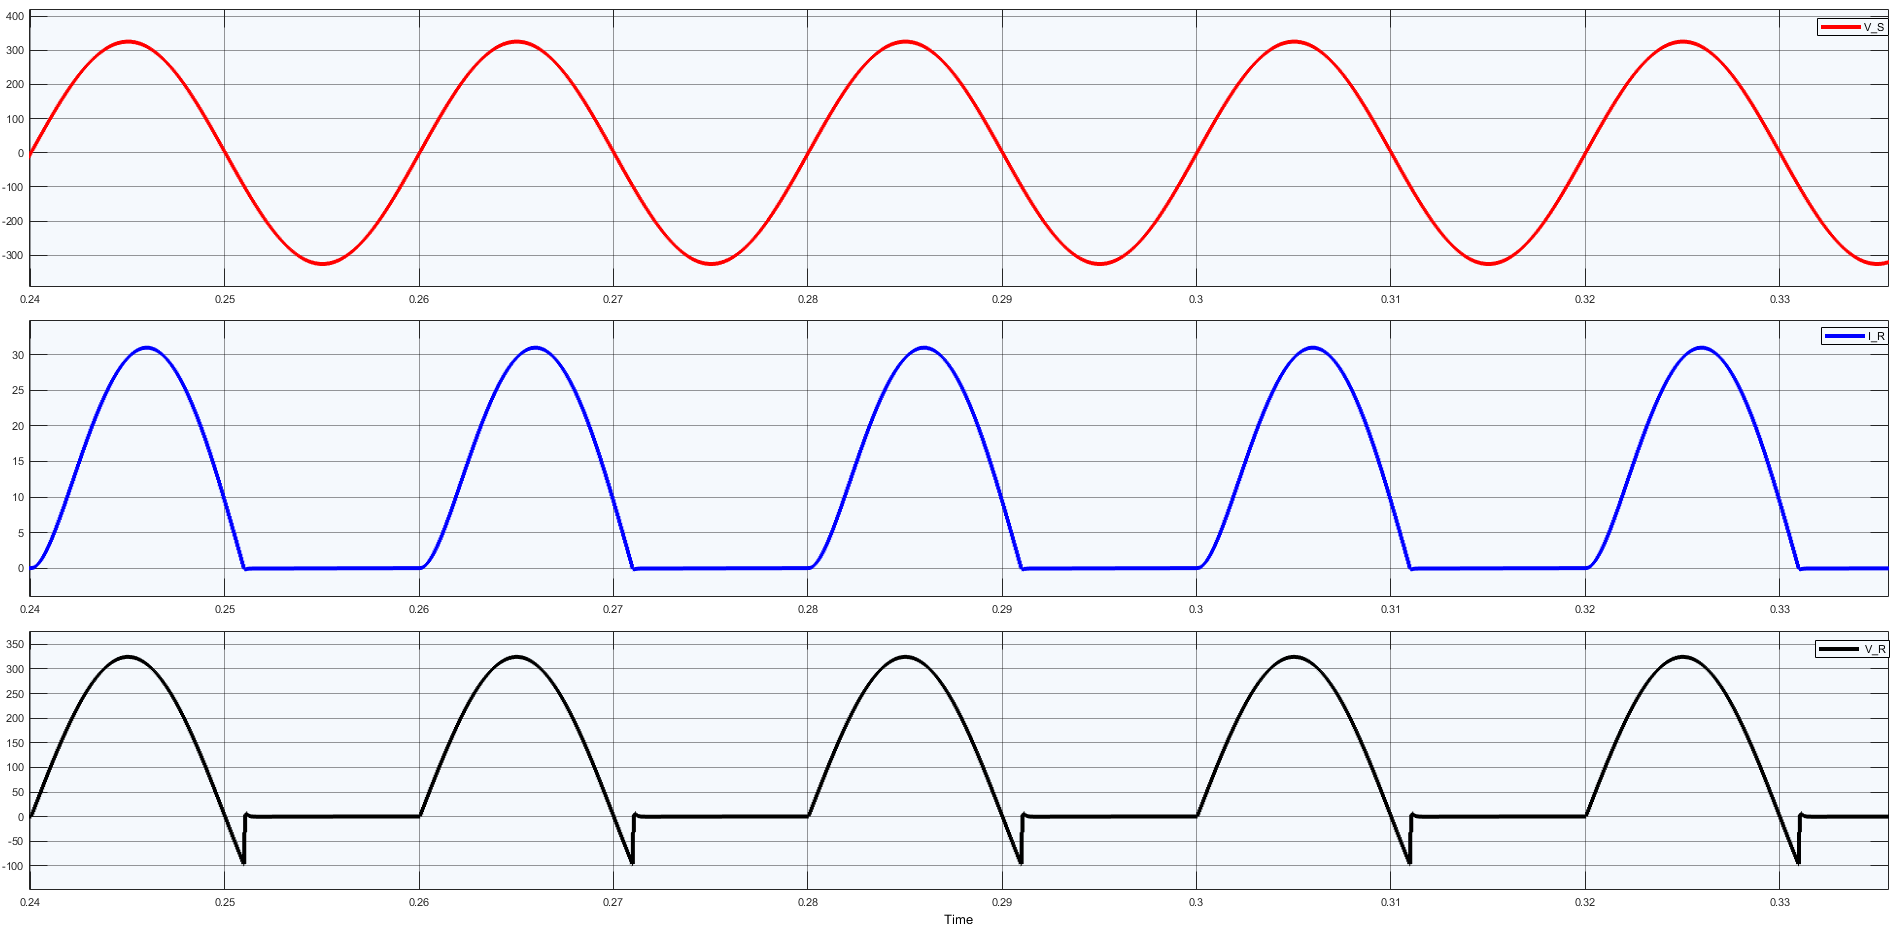
\includegraphics[width=1\textwidth]{images/experiment-1/circuit-scope-simulation-02.png}
    \caption{Scope Waveforms for Single Phase Half Wave Uncontrolled Rectifier with RL load}
    \label{Fig_waveform_single-phase-half-wave-uncontrolled-rectifier-with-RL-load}
\end{figure}

\pagebreak
